\setcounter{section}{4}
\setcounter{subsection}{21} % 4.22
\subsection{Link State Routing (1)}

\begin{enumerate}[(a)]
    \item Vervollst"andigen Sie den Graphen mit s"amtlichen Kanten und Kosten.

        Siehe Abbildung~\ref{fig:4.22.a}

    \item Verwenden Sie den Algorithmus von Dijkstra, um den kürzesten Pfad von
        A zu allen anderen Knoten zu finden, indem Sie die vorgegebene Tabelle
        ausfüllen.

        \begin{table}[h]
            \centering
            \begin{tblr}{
              cell{1}{2} = {c=3}{c},
              cell{1}{5} = {c=3}{c},
              cell{1}{8} = {c=3}{c},
              cell{1}{11} = {c=3}{c},
              cell{2}{1} = {c},
              hlines,
              vlines,
            }
                                                          & Schritt 1                               &                                      &                                              & Schritt 2                               &                                      &                                              & Schritt 3                               &                                      &                                              & Schritt 4                               &                                      &                                              \\
                \begin{sideways}Ziel-Knoten\end{sideways} & \begin{sideways}Vorgänger\end{sideways} & \begin{sideways}Kosten\end{sideways} & \begin{sideways}Schon Besucht?\end{sideways} & \begin{sideways}Vorgänger\end{sideways} & \begin{sideways}Kosten\end{sideways} & \begin{sideways}Schon Besucht?\end{sideways} & \begin{sideways}Vorgänger\end{sideways} & \begin{sideways}Kosten\end{sideways} & \begin{sideways}Schon Besucht?\end{sideways} & \begin{sideways}Vorgänger\end{sideways} & \begin{sideways}Kosten\end{sideways} & \begin{sideways}Schon Besucht?\end{sideways} \\
                A                                         & .                                       & 0                                    & (x)                                          & .                                       & 0                                    & (x)                                          & .                                       & 0                                    & (x)                                          & .                                       & 0                                    & (x)                                          \\
                B                                         & A                                       & 5                                    &                                              & C                                       & 4                                    &                                              & D                                       & 3                                    &                                              & D                                       & 3                                    & (x)                                          \\
                C                                         & A                                       & 1                                    &                                              & A                                       & 1                                    & (x)                                          & A                                       & 1                                    & (x)                                          & A                                       & 1                                    & (x)                                          \\
                D                                         & A                                       & 3                                    &                                              & C                                       & 2                                    &                                              & C                                       & 2                                    & (x)                                          & C                                       & 2                                    & (x)
            \end{tblr}

            \caption{}
        \end{table}

    \item Geben Sie f"ur den Knoten A die komplette Wegenwahltabelle an.

        \begin{table}[h]
            \centering
            \begin{tabular}{|c|c|c|}
                \hline
                Destination & Kosten & Next Hop \\
                \hline
                A           & 0      & .        \\
                \hline
                B           & 3      & C        \\
                \hline
                C           & 1      & C        \\
                \hline
                D           & 2      & C        \\
                \hline
            \end{tabular}
            \caption{}
        \end{table}
\end{enumerate}

\begin{figure}[p]
    \centering
    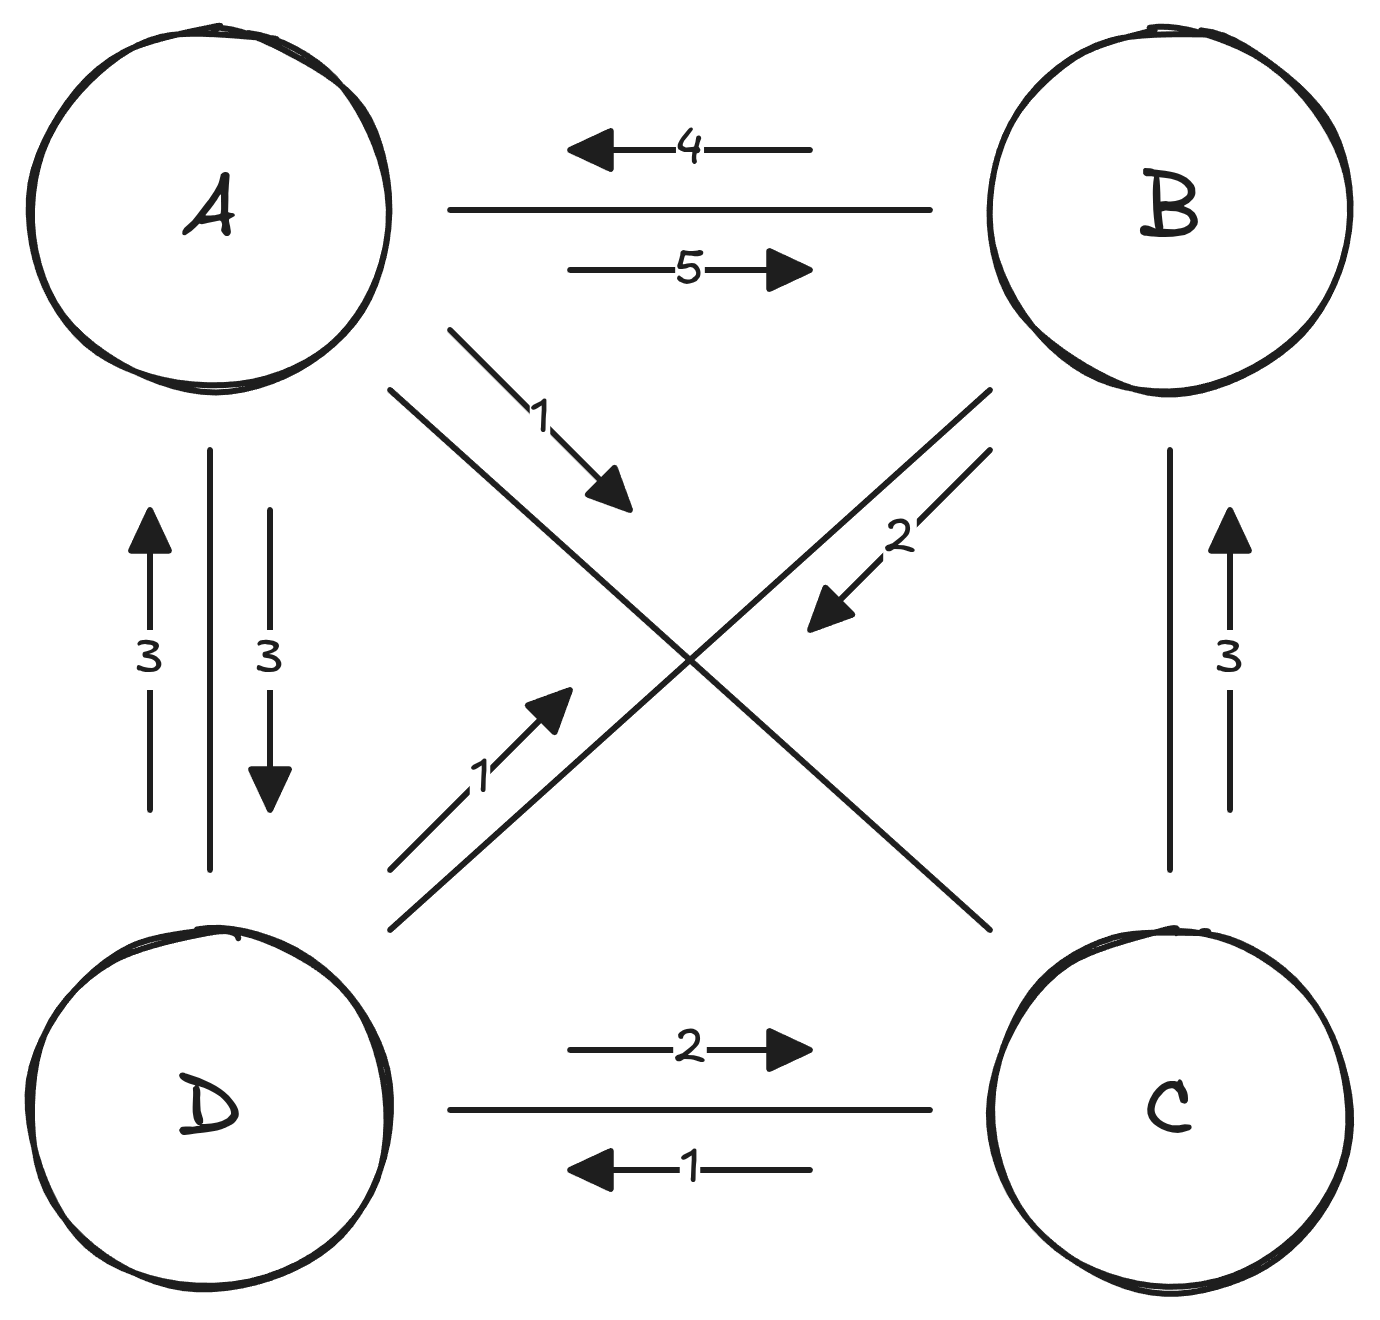
\includegraphics[width=1\textwidth]{./assets/4.22.a.png}
    \caption{}
    \label{fig:4.22.a}
\end{figure}

\FloatBarrier
